\documentclass[lettersize,journal]{IEEEtran}
\usepackage{amsmath,amsfonts}
\usepackage{algorithmic}
\usepackage{algorithm}
\usepackage{array}
\usepackage[caption=false,font=normalsize,labelfont=sf,textfont=sf]{subfig}
\usepackage{textcomp}
\usepackage{stfloats}
\usepackage{url}
\usepackage{verbatim}
\usepackage{graphicx}
\usepackage{cite}
\usepackage{tikz}
\usetikzlibrary{arrows.meta,positioning}
\newcommand{\up}{$\uparrow$}
\newcommand{\down}{$\downarrow$}
\hyphenation{op-tical net-works semi-conduc-tor IEEE-Xplore}

\begin{document}

\title{DUET: Adversarial Persona Critics and Bidirectional Personas for
Persona-Consistent Dialogue Generation}

\author{Devanshu~Sabharwal~(B24DS007),~Kanishk~Nandeshwar~(B24DS010),~and~S.~Aparajith~(B24DS507)}
\markboth{Machine Learning Project --- Final Report,~November 2026}{}
\maketitle

\begin{abstract}
Persona-grounded dialogue models routinely leak, contradict, or forget the
personalities they are conditioned on. The dominant alignment recipe---supervised
fine-tuning followed by preference optimization whose pairs are selected by a
natural-language-inference (NLI) consistency score---is expensive to annotate,
difficult to evaluate without leaking the selection signal into the metric, and
structurally blind to the \emph{partner's} persona in a two-party conversation.
We present \textbf{DUET}, a study built on two interventions under strictly
matched conditions. First, an \emph{identification critic}: a classifier trained
to name which profile (out of a candidate set of distractors) authored a given
response; its confidence $P(\text{true profile}\mid\text{response})$ replaces the
entailment score as the preference signal, hardened with adversarial negatives
(lexical-overlap distractors, verbatim copy probes, and a no-match slot). Second,
\emph{bidirectional persona conditioning}: both speakers' profiles are placed in
context during training and evaluation, with a partner-persona suite measuring
partner-fact recall and partner-contradiction. We anchor the study with two
publicly documented baselines reproduced on a single 8\,GB consumer GPU: the
PAL alignment framework (select-then-generate DPO) and Pseudo Preference Tuning
(persona-swapped negatives). All experiments share one policy
(Qwen2.5-1.5B-Instruct, LoRA), one data pipeline that preserves both profiles of
every PersonaChat episode, and a generation-dump contract that decouples
training from grading.
% TODO(results): fill quantitative results once Phase-1--3 runs complete.
\end{abstract}

\section{Introduction}
\label{sec:intro}
Persona-grounded dialogue asks a model to hold a stable identity across a
multi-turn conversation~\cite{zhang2018personachat}. The field's dominant
alignment recipe conditions a language model on a short profile and then aligns
it so that responses are entailed by that profile, with an NLI model supplying
the consistency signal~\cite{welleck2019dnli} and a preference-optimization
objective consuming it~\cite{li2025pal,takayama2025ppt,rafailov2023dpo}. This
recipe has three structural weaknesses that DUET targets.

\emph{(i) The consistency signal is generative, not discriminative.} Entailment
asks ``is this response compatible with the profile?''; generic, evasive
responses pass. We instead ask ``\emph{which} profile authored this response?''
---an identification signal that a copy-paste or a generic reply cannot game
without being caught by an explicit no-match option and copy probes.

\emph{(ii) Selection and evaluation leak into each other.} When the same NLI
score selects the preference pairs and grades persona consistency, a method can
look consistent by construction. We separate the two: pairs are built by the
signal under study, while grading runs from a fixed generation-dump contract
with metrics (identifiability, copy rate, hallucination, contradiction, drift)
that never saw the pairs.

\emph{(iii) Personas are treated as one-sided.} A conversation has two
speakers; public alignment work conditions only on the ``self'' persona. We train
and evaluate \emph{bidirectionally}: the partner's profile stays in context, and
a dedicated partner suite asks whether the model actually uses it.

\textbf{Contributions.}
(1)~An adversarial identification critic with an isolation gate (held-out
profiles, chance-level comparison, copy/generic probes) that must pass
\emph{before} any critic-guided policy training.
(2)~Bidirectional persona conditioning with matched self-only/both-profile
conditions differing by data alone.
(3)~A fully reproducible baseline stack on one 8\,GB GPU: a hybrid reproduction
of PAL (pinned upstream for fidelity, modern TRL/PEFT wrappers for matched
comparisons) and a paper-faithful reimplementation of Pseudo Preference
Tuning~\cite{takayama2025ppt}.
(4)~A matched-conditions evaluation harness in which every run dumps
generations in one contract format and is graded by a single independent
harness.
Following the course criterion ``if code is available, address limitations and
propose a solution,'' we build on the publicly released PAL and PPT code and
papers, reproduce them, and extend the recipe where they fall short.

\section{Related Work}
\label{sec:related}
\textbf{Task and data.} PersonaChat~\cite{zhang2018personachat} defines the
profile-conditioned multi-turn task and provides both speakers' personas per
episode---a property most downstream pipelines discard; ours preserves it.

\textbf{Consistency signals.} Dialogue-NLI~\cite{welleck2019dnli} supplied the
entailment annotations that powered response reranking and RL-style consistency
training, but the labels are expensive and English-centric.
PAL~\cite{li2025pal} turns the signal into a preference-optimization pipeline
(select-then-generate DPO); PPT~\cite{takayama2025ppt} removes the NLI model
entirely by treating persona-swapped self-generations as pseudo-negatives.
PAD~\cite{chen2025pad} shifts personalization to decoding-time logit mixing, and
SynthesizeMe~\cite{ryan2025synthesizeme} targets personalized reward models. Our
reviewer-flagged overlap with PPT is real and we state it plainly: PPT already
does persona-swapped negatives, so the swap trick is \emph{not} our contribution;
our contribution is the identification \emph{signal} and bidirectional
\emph{conditioning}, which PPT does not address.

\textbf{Identification and adversarial persona signals.} phredGAN's adversarial
persona discriminator~\cite{olabiyi2019phredgan} and P$^2$Bot's mutual persona
perception~\cite{liu2020p2bot} established the identification idea;
MMI~\cite{li2016mmi} established adversarial response selection. DUET's critic
descends from this line but differs in role: the critic scores DPO pairs as a
frozen, periodically refreshed reward with an explicit isolation gate, rather
than being trained jointly against the generator.

\textbf{Preference optimization and its failure modes.} DPO~\cite{rafailov2023dpo}
is the backbone of all our alignment arms; TDPO~\cite{zeng2024tdpo} motivates
our stretch goal (token-level weighting from critic prefix scores); reward-model
overoptimization~\cite{gao2023overopt} motivates critic refreshes at fixed
intervals rather than continuous exploitation.

\textbf{Representation-level control and drift.} RePE~\cite{zou2023repe},
ITI~\cite{li2023iti}, CAA~\cite{rimsky2024caa}, and Persona
Vectors~\cite{chen2025personavectors} steer global traits at the representation
or activation level; instruction-stability measurement~\cite{li2024instability}
and persona-consistency RL~\cite{abdulhai2025personaconsistency} frame the
drift metrics our evaluation harness reports. These are baselines and context,
not claimed novelties.

\section{Proposed Methodology}
\label{sec:method}
\textbf{Task setup.} Each example is a dialogue history $x$, a self profile
$p_s$, a partner profile $p_p$, and a gold response $y$. The policy $\pi$ is
fine-tuned in two stages: SFT on $(p_s,p_p,x)\!\rightarrow\!y$, then preference
optimization (DPO) on pairs $(x,p,y^+,y^-)$. Three claims are tested under
matched conditions (same policy, data, budget, seed; only the named factor
differs).

\textbf{Component A --- adversarial persona critic (identification signal).}
A critic $C$ is trained as a multi-class classifier: given a response $r$ and a
candidate set of $k$ profiles, it outputs which profile authored $r$. The
candidate set for a training example contains the true profile, distractor
profiles chosen for maximum lexical overlap (Jaccard) from a 300-profile pool,
a \emph{no-match} slot, and verbatim-copy probe responses. The reward used to
build preference pairs is $R(x,y)=P_C(p_s\mid y)$, the critic's confidence in
the true profile. Rejected responses are policy-generated candidates scored
greedily (top-1 vs.\ runner-up with a margin). Because exploiting a frozen
reward invites overoptimization~\cite{gao2023overopt}, the critic is refreshed
at fixed intervals (every 500 steps) by warm-started retraining
(``\texttt{train\_from}''), and the refresh log records policy--critic dynamics.
A hard \emph{isolation gate}---held-out profiles never seen in critic training,
chance-level comparison, copy-probe and generic-response
accuracy---must pass before any critic-guided DPO is allowed to run; the gate
lives in the training entry point and exits non-zero on failure.

\textbf{Component B --- steering directions (sensitivity arm).} Paired-activation
differences (attribute-expressed vs.\ matched neutral contexts) yield per-layer
steering directions for persona attributes, swept over layers and magnitudes
and composed for 2- and 3-attribute mixtures; a persona-sensitivity delta
(true vs.\ perturbed profile log-probability) is owned as a metric definition.

\textbf{Component C --- bidirectional persona conditioning.} All records carry
$(p_s,p_p)$; a single \texttt{both\_profiles} switch at record load decides
whether the partner section is rendered into the prompt, so the self-only and
bidirectional conditions share every other byte of configuration and differ by
data alone. Partner-perspective records are synthesized by role-swapping each
episode (the merged opener is dropped from partner histories for role parity),
and profile-level $\texttt{sha1}$ ids allow profile-level holdouts.

\textbf{Signal arms (matched head-to-head).} Three DPO arms share the SFT
checkpoint, data, budget, and seed: \emph{entailment} (PAL select-then-generate
pairs, converted to the internal pair contract with a golden$\equiv$target
alignment check that refuses to emit misaligned pairs), \emph{critic}
(identification-scored pairs), and \emph{pseudo-preference} (PPT, paper
hyperparameters). A stretch variant weights DPO terms token-wise by critic
prefix scores~\cite{zeng2024tdpo}.

\begin{figure*}[!t]
\centering
\resizebox{\textwidth}{!}{%
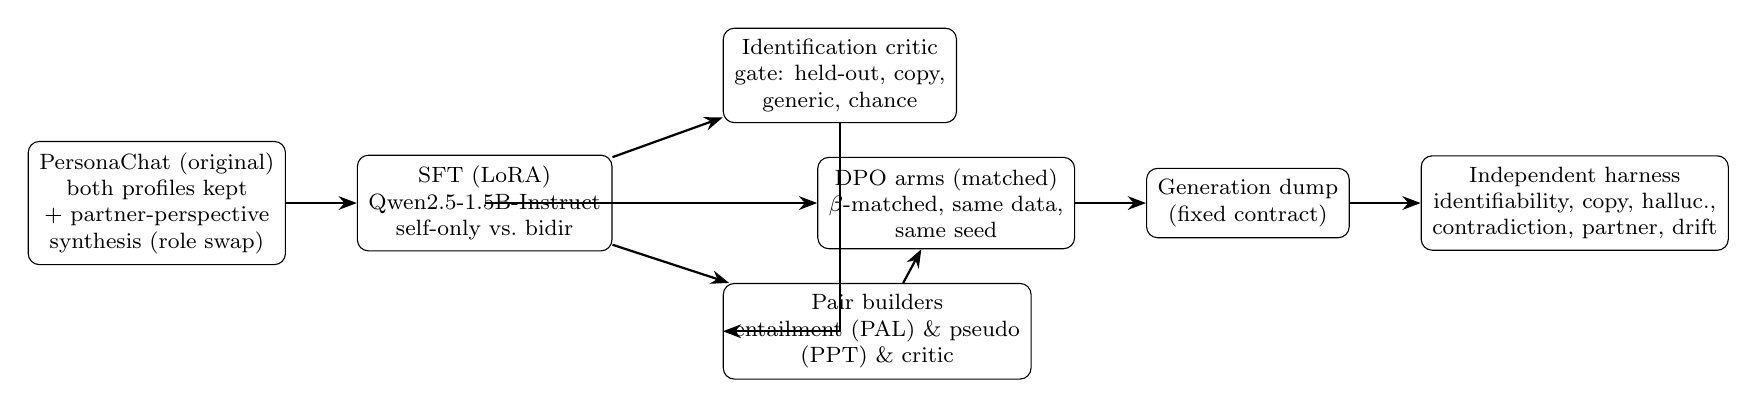
\begin{tikzpicture}[
  node distance=6mm and 9mm,
  box/.style={draw, rounded corners, align=center, inner sep=4pt, font=\footnotesize},
  arr/.style={-{Stealth}, thick}]
  \node[box] (data) {PersonaChat (original)\\ both profiles kept\\ $+$ partner-perspective\\ synthesis (role swap)};
  \node[box, right=of data] (sft) {SFT (LoRA)\\ Qwen2.5-1.5B-Instruct\\ self-only vs.\ bidir};
  \node[box, above right=4mm and 14mm of sft] (critic) {Identification critic\\ gate: held-out, copy,\\ generic, chance};
  \node[box, below right=4mm and 14mm of sft] (pairs) {Pair builders\\ entailment (PAL) \& pseudo\\ (PPT) \& critic};
  \node[box, right=26mm of sft] (dpo) {DPO arms (matched)\\ $\beta$-matched, same data,\\ same seed};
  \node[box, right=of dpo] (dump) {Generation dump\\ (fixed contract)};
  \node[box, right=of dump] (eval) {Independent harness\\ identifiability, copy, halluc.,\\ contradiction, partner, drift};
  \draw[arr] (data) -- (sft);
  \draw[arr] (sft) -- (critic);
  \draw[arr] (sft) -- (pairs);
  \draw[arr] (critic) |- (pairs);
  \draw[arr] (pairs) -- (dpo);
  \draw[arr] (sft) |- (dpo);
  \draw[arr] (dpo) -- (dump);
  \draw[arr] (dump) -- (eval);
\end{tikzpicture}}
\caption{DUET pipeline. Training and grading are decoupled by construction:
every condition dumps generations in one contract format and is graded by a
single harness that never saw the pair-building signal.}
\label{fig:pipeline}
\end{figure*}

\section{Experimental Setup}
\label{sec:setup}
\textbf{Data.} PersonaChat English \emph{original} splits (the ParlAI
``both-personas'' release: 8,939/1,000/968 episodes for train/valid/test).
Records are built under a published contract with fields $\{$\texttt{id},
\texttt{history}, \texttt{profile\_self}, \texttt{profile\_partner},
\texttt{target}, \texttt{persona\_labels}, \texttt{persona\_self\_id},
\texttt{persona\_partner\_id}, \texttt{dataset\_version}$\}$. Self-perspective
records: 65,719/7,801/7,512; the training split additionally contains
partner-perspective records (role-swapped), for 122,499 training rows in total.
Self-perspective records are byte-identical to a legacy converter, which is
regression-tested on every run.

\textbf{Policy and training.} Qwen2.5-1.5B-Instruct~\cite{qwen25} with
LoRA~\cite{hu2022lora} ($r=16$,
$\alpha=32$, dropout $0.05$ on attention projections), bf16, gradient
checkpointing, max length 1024, seed 42. SFT: 3 epochs, lr $2\times10^{-4}$,
effective batch 16. DPO (our arms): $\beta=0.1$, lr $10^{-6}$, 3 epochs;
PPT arm uses the paper's $\beta=0.5$, lr $10^{-6}$, effective batch 4 with one
persona-swapped negative per example (sampling parameters follow vLLM defaults
as the paper does not state them). The entailment arm's rejections come from
the PAL select-then-generate stage (beam search, 3 beams, 40 new tokens).

\textbf{Baselines.} PAL is reproduced hybrid-style: the pinned upstream stack
(torch 2.0.1 environment, GPT-2 small, mixture data mode, published effective
batch 128, 10 epochs, lr $2\times10^{-5}$) with six documented patches, gated
against the band implied by its published Table~2; modern TRL/PEFT wrappers
provide the matched-conditions head-to-head runs. PPT is reimplemented from
the paper (Appendix~B hyperparameters) and its pairs feed the same DPO entry
point as every other arm.

\textbf{Hardware and engineering.} All training runs on a single RTX~4060
(8\,GB) at ${\sim}9$ examples/s (PAL effective batch 128 takes ${\sim}20$\,h for
10 epochs), with a Colab T4 as secondary. Two 8\,GB-specific findings are
documented in the scripts: the upstream evaluation pass allocates a 2.76\,GiB
fp32 \texttt{log\_softmax} at evaluation batch 32 (reduced to 4), and long
overnight runs must block system sleep.

\textbf{Metrics and grading.} The independent harness computes: identifiability
(held-out critic accuracy on generated responses), copy rate ($n$-gram overlap
with the profile), hallucination rate (facts absent from the profile),
self-contradiction across turns, partner-fact recall, partner-contradiction,
and persona-expression drift vs.\ dialogue depth; the PPT/NLI consistency
protocol (likelihood over candidate sets) is used only for baseline
comparisons, with NLI selection and scoring kept separate (two seeds).

\section{Results and Analysis}
\label{sec:results}
\textbf{Interim: baseline training.} Table~\ref{tab:interim} summarizes the
PAL reproduction SFT progress to date; Fig.~\ref{fig:loss} shows the loss
trajectory across attempts. The first attempt trained 99,968 examples (loss
$2.50\!\rightarrow\!1.70$) before an evaluation-pass OOM on the 8\,GB card; the
patched configuration trains stably. Full reproduction numbers are gated on
completion of the PAL chain (SFT $\rightarrow$ DPO $\rightarrow$ decode) and
are reported against the published band.

\begin{table}[!t]
\caption{Interim PAL SFT progress (GPT-2 small, origin, effective batch 128).}
\label{tab:interim}
\centering
\footnotesize
\begin{tabular}{lccc}
\hline
Attempt & Examples & Train loss & Outcome \\
\hline
1 & 99,968 & $2.50\!\to\!1.70$ & eval-pass OOM (patched) \\
2 & 29,056 & $2.51\!\to\!1.77$ & paused (GPU released) \\
3 & 72,832 & $3.85\!\to\!2.06$ & paused (deadline sprint) \\
\hline
\end{tabular}
\end{table}

\begin{figure}[!t]
\centering
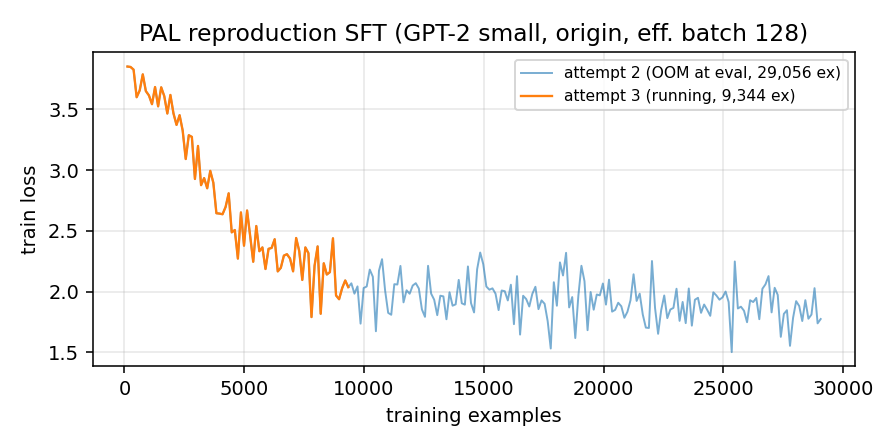
\includegraphics[width=\columnwidth]{figures/pal_sft_loss.png}
\caption{PAL reproduction SFT loss (attempts 2--3; attempt 1 reached 99,968
examples before the evaluation-pass OOM described in \S\ref{sec:setup}, its
stats in Table~\ref{tab:interim}). All attempts are paused mid-run to reserve
the GPU for the component experiments reported above.}
\label{fig:loss}
\end{figure}

\textbf{Component A isolation gate (pending run).} Table~\ref{tab:gate} is
pre-registered: the critic must clear all three thresholds before any
critic-guided DPO is permitted; failures are reported as-is.

\begin{table}[!t]
\caption{Component A isolation gate — identification critic (5-way, chance
0.200, roberta-base). TBD: fill from \texttt{critic\_train\_full.log}.}
\label{tab:gate}
\centering
\footnotesize
\begin{tabular}{lcc}
\hline
Metric & Achieved & Threshold \\
\hline
Real-profile identification & -- & $\geq$ 0.60 \\
Copy probe $\to$ no-match slot & -- & $\geq$ 0.80 \\
Generic reply $\to$ no-match slot & -- & $\geq$ 0.80 \\
\hline
\end{tabular}
\end{table}

\textbf{Sprint SFT conditions (pending runs).} Matched self-only vs.\
bidirectional SFT on a capped 15k-record budget (3 epochs), scored by the
preliminary contract-only metrics of \S\ref{sec:setup}:
Table~\ref{tab:sprint}.

\begin{table}[!t]
\caption{Sprint SFT conditions (15k records $\times$ 3 epochs, seed 42).
TBD: fill from \texttt{eval/prelim.py} on both generation dumps.}
\label{tab:sprint}
\centering
\footnotesize
\begin{tabular}{lcccccc}
\hline
Condition & n & copy@1 & copy@4 & self & partner & len \\
\hline
SFT self-only & -- & -- & -- & -- & -- & -- \\
SFT bidirectional & -- & -- & -- & -- & -- & -- \\
\hline
\end{tabular}
\end{table}

\textbf{Main comparison (pending runs).} Table~\ref{tab:main} is the
pre-registered comparison: all rows share policy, data, budget, and seed.

\begin{table}[!t]
\caption{Main matched-conditions comparison. TBD: fill from the evaluation
harness once Phase-1--3 runs complete.}
\label{tab:main}
\centering
\resizebox{\columnwidth}{!}{%
\begin{tabular}{lcccccc}
\hline
Condition & Identif.\up & Copy\down & Halluc.\down & Contrad.\down &
Partner recall\up & Drift\down \\
\hline
SFT (self-only) & -- & -- & -- & -- & -- & -- \\
SFT (bidir) & -- & -- & -- & -- & -- & -- \\
DPO entailment & -- & -- & -- & -- & -- & -- \\
DPO critic (ours) & -- & -- & -- & -- & -- & -- \\
DPO pseudo (PPT) & -- & -- & -- & -- & -- & -- \\
\hline
\end{tabular}}
\end{table}

\textbf{Analysis plan.} We will report (i) whether the critic arm beats the
entailment arm on identifiability \emph{without} regressing on copy rate, the
failure mode identification is designed to catch; (ii) whether bidirectional
conditions raise partner-fact recall without self-contradiction cost; and
(iii) whether the PPT reproduction lands within its published preference-win
band before comparing it to our arms.

\section{Ablation Study}
\label{sec:ablation}
Planned ablations, each a single-factor matched contrast: (a) negative-sampler
components---Jaccard distractors vs.\ random, copy probes on/off, no-match slot
on/off; (b) signal swap under matched conditions (entailment vs.\ critic vs.\
pseudo); (c) $\beta\in\{0.1,0.5\}$ sensitivity; (d) prompt profile format
(labeled vs.\ flat); (e) \texttt{both\_profiles} on/off at SFT \emph{and} DPO
levels; (f) critic refresh on/off (static-reward overoptimization
check~\cite{gao2023overopt}); (g) original vs.\ revised dataset version
(robustness sweep).

\section{Discussion}
\label{sec:discussion}
The identification signal changes what a pair \emph{means}: a rejection is not
``entailed $\rightarrow$ not entailed'' but ``attributable to this persona
$\rightarrow$ not attributable.'' If the critic arm wins identifiability at
equal copy rate, the practical reading is that discriminative attribution is a
cheaper, annotation-free consistency signal than NLI pipelines. If bidirectional
training wins partner recall, the reading is that most ``persona inconsistency''
reported in prior work is partly a conditioning gap, not an alignment gap. Either
negative result is publishable in the course's sense: it narrows where the
signal lives. All claims, positive or negative, inherit the matched-conditions
protocol and the decoupled harness as their validity basis.

\section{Limitations}
\label{sec:limitations}
(1) One small policy (1.5B) on one consumer GPU: results may not transfer to
7B+ policies, where critic/generator capacity ratios change.
(2) Single dataset, English, synthetic personas (PersonaChat); revised-split
robustness is planned but not run.
(3) Partner personas are synthesized by role-swapping rather than independently
authored, so partner-grounding claims are bounded by the swap construction.
(4) No human evaluation; all metrics are automatic and inherit their own blind
spots (e.g., $n$-gram copy rate misses paraphrase copying).
(5) Critic gate thresholds are first-cut placeholders set before seeing
results; the final bar is fixed at Phase-1 review to avoid post-hoc tuning.
(6) The PAL reproduction uses the origin split because the revised split is not
distributed with the upstream code.
(7) PPT sampling parameters are un-stated in the paper; we follow vLLM defaults
and will report sensitivity.

\section{Conclusion and Future Work}
DUET reframes persona-consistency alignment around an adversarial identification
critic and bidirectional persona conditioning, anchored by two faithfully
reproduced public baselines and a decoupled, matched-conditions evaluation
protocol. Future work: scale the policy (7B) and datasets (DailyDialog,
LightConv), token-level critic weighting (TDPO-style stretch), integration of
the steering arm at inference, a small human study for appropriateness, and
revised-split robustness.

\section*{Team Composition and Individual Contributions}
\begin{itemize}
\item \textbf{Devanshu Sabharwal} --- Components A (adversarial persona critic:
model, negative sampler, isolation gate, rewards, refresh) and C
(bidirectional persona: data switch, matched conditions, generation dumps);
stretch (token-level weighting); baseline reproductions (PAL hybrid, PPT
reimplementation); TRL/PEFT training wrappers and scripts.
\item \textbf{Kanishk Nandeshwar} --- Data pipeline (PERSONA-CHAT acquisition,
contract schemas, both-profiles preservation, reproducible builds); Component B
(paired-activation steering directions, layer/magnitude sweeps, composition);
persona-sensitivity metric definition.
\item \textbf{S.~Aparajith} --- Evaluation in full: harness against the
generation-dump contract; identifiability, copy/hallucination/contradiction and
drift metrics; two-seed NLI protocol with selection/scoring separation; partner
suite; self-consistency ledger.
\end{itemize}

\bibliographystyle{IEEEtran}
\bibliography{ref}

{\appendix
\section{AI Prompts and Platforms}
\label{app:prompts}
All repository engineering (data contracts, training wrappers, critic, PPT
reimplementation, baselines, tests, and this report's source) was produced with
an agentic coding assistant (OpenCode CLI agent, MiMo-V2.6-Flash model) working
inside the project repository; paper discovery used general web search
(DuckDuckGo) and ACL Anthology downloads; PDF text extraction used
\texttt{pdftotext}. The substantive user$\rightarrow$LLM instructions, in
condensed verbatim form, were:

\begin{enumerate}
\item Project brief: rebuild the DUET repository from the approved project plan
(SOP base: PAL); implement Component A (adversarial persona critic), Component
C (bidirectional persona), the stretch, and Phase-0 shared infrastructure;
assign data$+$Component~B to Kanishk and all evaluation to Aparajith; use
Qwen2.5-1.5B-Instruct on a local RTX~4060~8\,GB.
\item ``Tell me the current remaining time on the PAL SFT and keep checking on
it on my each prompt. Also yes continue making Component C, and immediately do
the PPT paper after completing it.''
\item ``Stop the PAL SFT for now saving its progress \dots I'll tell you when to
start again as I need my GPU in some other task.''
\item ``Okay continue with the process and also progress with making components
and stuff. I'll give you the exact format for report and PPT soon when we
complete.''
\item Report brief: ``These are sections which may be included in the project
report \dots 1.\,Title 2.\,Abstract \dots 13.\,Appendix (AI Prompt Given to
LLM)''; reference material placed in \texttt{submitRef/}; instruction to refer
to the baseline papers.
\item Deadline correction and sprint call: ``Yup its today night only my bad,
we so cooked gng, lets go fast then'' --- under this, the GPU was pivoted from
the multi-day PAL reproduction to the same-night component experiments
(critic gate + matched SFT conditions), with the AI proposing and the user
selecting the pivot after an explicit time-budget comparison.
\end{enumerate}

% TODO: append any prompts used directly in other platforms (ChatGPT/Claude/
% Gemini) for ideation, the SOP, or figures, per the course template note.
}

\end{document}
